%----------------------------------------------------------------------------------------
%	PACKAGES AND DOCUMENT CONFIGURATIONS
%----------------------------------------------------------------------------------------

\documentclass[a4paper,twoside,12pt]{report}
\usepackage[toc,page]{appendix}
\usepackage{booktabs}
\usepackage{graphicx} % Required for the inclusion of images
\usepackage{amsmath} % Required for some math elements
\usepackage[top=1.0in,bottom=1.0in,left=1.0in,right=1.0in]{geometry}  %bindingoffset=1in	 
%\setlength\parindent{10pt} % Removes all indentation from paragraphs
%\renewcommand{\labelenumi}{\alph{enumi}.} % Make numbering in the enumerate environment by letter rather than number (e.g. section 6)
\usepackage{float}
\usepackage[english]{babel}
\usepackage{hyperref}
%\usepackage{times}
\usepackage{setspace}
\usepackage{float}
\usepackage{subcaption}
\usepackage{graphicx}
\usepackage{mathptmx} %for times new roman
\usepackage{titlesec}
\titleformat{\chapter}[display]
{\bfseries\Huge\centering}{\chaptertitlename\ \thechapter}{18pt}{\Huge}
\titleformat{\section}
  {\Large\bfseries}{\thesection}{12pt}{}
\titleformat{\subsection}
  {\large\bfseries}{\thesubsection}{11pt}{}
\begin{document}
\pagenumbering{roman}
\begin{spacing}{1}  %single spacing for abstract
\begingroup
\fontsize{12pt}{14pt}\selectfont
\begin{center}
	\Huge\bfseries
	\textit{Abstract}
\end{center}
\vspace{0.3in}
\textit{
\textbf{Keywords:} 
}
\endgroup
\end{spacing}
\begin{spacing}{1.5}
\tableofcontents
\listoffigures
\listoftables
\chapter{Introduction}
Blockchain facilitates to transfer value without the need for a intermediate party. Examples of such values are information, contracts, assets, identity. This technology gives cryptographically secure and decentralized mechanism that removes the need of management from single entity. Blockchain technology is building block for the cryptocurrencies such as Bitcoin and Ethereum. It is efficiently shared, trusted, and secure ledger of various transactions.  
\par
The traditional approach for payment methods and storage purposes are in a centralized manner. Trusted third party is required for electronic banking transaction. The intervention of the third entity makes transaction slower and expensive, and even high cost is needed to make an irreversible transaction. To tackle this issue, a system is required, which have features like publicly available, free inference of third party, computationally infeasible reverse and more importantly secure.  In October 2008, Satoshi Nakamoto published for peer-to-peer distributed technology which can fulfil all these requirements preciously. It uses cryptographic proof rather than a trusted third party, which enable entities two to participate directly. This advanced technology is secure as far as a single entity or organization doesn't control more than 50\% of network \cite{satoshinakamoto}. Immutability of ledger can be useful for saving data for a more extended period without risk of tamper.      
\pagenumbering{arabic}
\section{Motivation}
\section{Objective}
To give a lucid explanation of how blockchain works, potential risk and issues lurking on this technology.
\section{Applications}
\subsubsection{Cryptocurrency}
Omnipresent digital currency mechanism facilitated by Blockchain works automatically, it also facilitates a real-time, time-efficient transaction which might be next to impossible in traditional database system \cite{overviewofblockchainsecurity,democraticmininginbitcoins}. Use of cryptocurrency removes the requirement of the third party, which makes the whole system fast and reliable. It also enables banks banks to progress payment speedily and more preciously while reducing resource requirements.
Address of each node is also a cryptographic hash, which can hide the identity of a particular node.  Various feathers provided by Blockchain, makes it next-generation business process development.
\subsubsection{Health Care}
https://www.investopedia.com/terms/b/blockchain.asp
\subsubsection{Traffic Scene}
\subsubsection{Transaction Tracking}
\section{Report Outline}
\chapter{Background and Literature Survey}
\section{Types of System}
Every system can be divided into three category. First, centralized. Second, Decentralized, and third is Distributed. Differences in the system can affect every whoever is using it \cite{gfg_cent_vs_decent}. Simultaneous use of these three category is not possible. Hence, organizations and institutions need to choose out of available option. While deciding, which system to use, pros and cons of each system should be considered. With history's perspective,centralized system are more prominent. But centralized system has their own disadvantages which can be overcome by decentralized or distributed system. Below detail explanation of each system is given with its potential advantages and disadvantages.
\subsection{Centralized}
Centralized system is more easy to define, implement and more intuitive. Centralized system uses typical client/server architecture where unlimited number of client side nodes can communicate with one server side node. Every client nodes are connect to server node, so server node can be considered as central node, and central node is responsible for working as storage from where every client can access their information. 
Wikipedia, IBM are centralized systems. In which, user can search for a specific query, and that query will be resolved by server lying at possibly any corner of the world.
\subsubsection{Advantages}
\begin{enumerate}
\item{Quick, easy deployment and quick development}
\item{Easy maintenance of system as whole}
\item{Feasible to control data from central entity}
\item{Cost effective}
\item{Quick update}
\end{enumerate}
\subsubsection{Disadvantages}
	\begin{enumerate}
	\item{Network connectivity is key factor - Chances of system failure is higher, due to dependency on single server}
	\item{Longer access time for nodes residing at far points}
	\item{Difficult Server Maintenance because only one server}
\end{enumerate}	 
\subsection{Decentralized}
In this type of system, multiple central entities are available rather than single central entities, and these central entities are also connected to each other. Every central entities also stores a own copy of data. Presence of centralized still makes still vulnerable to accident as centralized one. However, architecture of decentralized system adds robustness, because even if central entity fails, rest of central entities still continue to work. It means, it allows system administrator to repair one central node, while system itself continue its work, with limitation on performance and data availability to some extent.   
\subsubsection{Advantages}
\begin{enumerate}
	\item{Access time is faster than centralized system}
	\item{High fault tolerance}
	\item{More flexible and diverse system}
	\item{Scalability is higher than centralized}
	\item{Easy evolution}
\end{enumerate}
\subsubsection{Disadvantages}
\begin{enumerate}
	\item{Security and privacy risk}
	\item{Higher maintenance cost}
\end{enumerate}
\subsection{Distributed}
Distributed system removes need of central entity, which ultimately rejects centralization. Each and user have equal access. However, access rights can be altered as when required. Blockchain and internet are well-known example of distributed system. It is free from independent failure. Apart from that, it also allows user to define ownership of data. Resources are distributed among users that leads to improved efficiency of network. Because of the benefits it provides, distributed framework is changing industry drastically.
\subsubsection{Advantages}
\begin{enumerate}
	\item{Transparency}
	\item{Scalable}
	\item{Easy evolution}
	\item{Extremely high fault tolerance}
\end{enumerate}
\subsubsection{Disadvantages}
\begin{enumerate}
	\item{Difficult to implement}
	\item{Higher maintenance cost}
\end{enumerate} 
\section{Blockchain Technology}
Blockchain is chain of digital blocks containing various data and information. Once a block is connected to the chain, it can never be changed again, and it will be publicly available to read. For connecting new block to chain, blockchain uses hashvalue of previous block and new block. Digital blocks contains information of hash of previous block, time and information which is to be added,etc. That is quite groundbreaking due to it avails facility for keeping track of medical records, full supply records and transaction records, etc. Some important terminologies are explained below.
\subsubsection{Nonce}
Blockchain allows only specific type of hash values. For an example, first ten digits should be zero only. It is not always the case that hash value will have ten digit in starting. In order to, meet up this requirement while finding eligible signature data in the string needs to be changed continuously. Moreover, hash functions are designed in such a way that only a trivial change in string can leads to complete different hash value. So, small special piece of data is added in the string to get acceptable hash value. That piece of data is known as nonce.   
\subsubsection{Mining Process and Miners}
\label{miningprocess}
The process of finding nonce is called mining. The entity which continuously work to find such nonces are known as miners. Methods that miners use can also be relate to trial and error method. Miners use their computation power for finding acceptable signature. Acceptable signature is expected output from any miner. Large computational power increases possibility of finding out proper nonce in lesser time. In the case of publicly available blockchain, any user can work as miner by using blockchain specific application. Process, in which, miners compete to get signature and get rewared for success is also known as Proof-of-Work \cite{satoshinakamoto}. Second method for choosing miner is called Proof-of-Stack. In Proof-of-Stack selection of miner depends on the cryptocurrency miner posses, rather than computational power which is used in Proof-of-Work \cite{saad_exploring_2019}. Other popular consensus algorithms are Practical Byzantine fault tolerance (PBFT), Proof-of-Reputation \cite{saad_exploring_2019}.
\begin{figure}[h!]
\begin{center}
  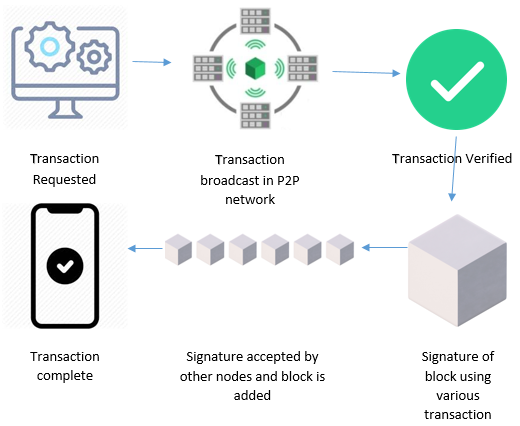
\includegraphics[width=0.8\linewidth]{images/workingofblockchain.png}
  \caption{Working of blockchain}
  \label{img: workingofblockchain}
\end{center}
\end{figure}  
\subsubsection{How Block is Added to ledger?}
According to Fig \ref{img: workingofblockchain}, whenever new data is to be added in blockchain, it is added in to the imaginary pool of unverified data. Miners who have participate in mining process can access those data from pool. Once miners get enough information that can create one block, they fetch data from pool, and start mining procedure as explained in section \ref{miningprocess}. As soon as miner find acceptable signature, it broadcast that signature in the system. Agreement from the predefined percentage of node is required. Once that many nodes agree for new block , new block is added to the ledger. Afterwards, block becomes immutable.
%\section{Different Hash Function}
%\subsection{SHA-256} Bitcoin is using this. 
\section{Features of Blockchain Technology}
\subsection{Robustness}
Myriads of computers all around the world keeps own copy of ledger, and availability of duplicate copies makes Blackchain robust to the failure of single (or a few) node \cite{satoshinakamoto}. Unavailability or instability of node doesn't stop whole system from working, because ledger still exists in other nodes. Alteration of data at one node is infeasible, it requires agreement or change in data on at least 50\% of node.
\subsection{Censorship-Resistance}
Absence of single entity which manipulates a blockchain, that is paramount feature of decentralized network. In centralized approach, one authority has access to whole database, and it can change database as and when required \cite{satoshinakamoto}. For an example, while doing bank transaction, third party is always involved. On other hand, blockchain abolish interference of centralized authority, which facilitates to do transaction directly between two parties.
\subsection{Transparency}
Each and every change in ledge also goes through every participants. Updates in database are reflected in every node, so that new information is available in trivial time. It means each node has knowledge about the data residing at other node. Data is also consistent with every node, it provides transparency to the system \cite{satoshinakamoto}.  
\subsection{Irreversibility}
Every transaction of ledger in blockchain, defines next transaction. In other word, every transaction contains hash value of previous transaction. It means that every block of chain is connected. So, for changing one block of ledger, all the previous transaction requires changes, that is infeasible task for today's computer. That characteristic makes blockchain irreversible and secure against potential threat.
%\subsection{Security Purposes}
%\subsection{Time Constraint}
%\subsection{Financial Saving}
\subsection{Disaster Recovery}
Synchronized storage of data at various node improves fault-tolerance and reliability of blockchain. Every node has a access to create data and store ledger of blockchain, but it comes the cost redundancy \cite{democraticmininginbitcoins,minerevolutioninbitcoinnetwork}.   
Moreover, attack on individual node can't cause destruction to the whole system \cite{fangfangdai}. 
%\subsection{Tamper Proofing}
%\cite{fangfangdai}
\section{Types of Blockchain}
On the basis of who can assess and control blockchain, this technology has two types of mechanism. First is permissionless blockchain is open for public use, whereas second one is permissioned blockchain which allows only limited number of users. Description and example of both type is explained below.       
\subsection{Permissionless Blockchain}
Permissionless Blockchain is also known as public Blockchain. Whole idea differs from the previous type. Any computer, with adequate technological requirements mandated by network,can participate as a minor. As name suggests, no other personal identity or machine authorization required to play a role of minor. It allows anyone to read and participate in system. When it is used as a part of cryptocurrency, at that time, having cryptocurrency is enough allow any user to transact digital money. This model is almost resembles basic idea of blockchain technology given by Satoshi Nakamoto \cite{satoshinakamoto}. On other hand, scalability and privacy issues are the drawbacks of public blockchain. To conclude, any entity can participate for transaction, and that can result into the privacy breach. Bitcoin and Ethereum are examples of permissionless blochain technology. 
\subsection{Permissioned Blockchain}
Blockchain was original developed as publicly available and free system, but permissioned blockchain is exactly contrasting. Permission from owner is required to take part in blockchain. It gives control in owner's hand, it also means that one entity can manipulate whole system. That right of possession allows authorities to do whatever want to do with system, and also enables to impose various access rights to other users. For an example, owner can restrict some node from reading information. Even validation procedure is done by only selected entities. That makes this model faster and scalable than public blockchain. As an epitome, USA based supermarket company Walmart is designing permissioned blockchain to track fruits and vegetables. On the top of it, some information regarding products will be publicly available. Moreover, private blockchain is becoming popular in industries such as supermarkets, agriculture and transportation etc.
\section{Current Research}
\cite{fangfangdai}
\chapter{Cybersecurity Attacks, Risk and Prevention}
\section{Types of Attacks and Prevention Measure}
\label{typesofattacks}
Attackers have stolen \$1 billion from cryptocurrency exchanges and various other platform \cite{topfiveblockchainsecurityissues}. It becomes vital to analyse such potential attacks which have affected users and validation nodes all over the world. Different methodology can be used for damaging blockchain, and various preventive measures are required to thwart effect of malicious attack \cite{blockchainthreatreport}. 
\subsection{Phishing}
Phishing is defined as malicious attempt to extracting information from users \cite{wiki:phishing}. It includes sensitive information such as bank details, username, password, etc. In short, phishing is stealing confidential data by  masquerading attackers as a trusted party. Phishing breaks confidentiality of information \cite{andryukhinphishing}. Email spoofing and messaging are prominent ways to expose any computer to this attack. For implementation of phishing, attackers mostly disguise themselves as a representative of reputed firm. In addition to that, attackers makes their own website or application by a name trivially different from the original one. By the use of email or message, address of this platform is sent to potential victim. For an example, institute called Block.one which developed EOS.IO blockchain during the 2018, has been the victim of phishing attack \cite{wiki:phishing}. Phishing group sent email with the intention of stealing wallet key. Unfortunately, attack was successful. 
\par
Clone phishing is a type of attack in which duplicate webpage with also most resembling, or webpage with approximately same is made \cite{andryukhinphishing,phishingkaspersky}. Targeted phishing one of the prominent type of attack. It includes aiming at owners of wallets, key person of companies, and owner of cryptocurrency \cite{aimedphising,andryukhinphishing}. Duplicate cryptocurrency purses uses forgery purse, in which applications related to cryptocurrency is published on well-known application providing platform. Then that malicious demands for the private key and purse password \cite{andryukhinphishing}.          
\subsubsection{Electrum Bitcoin}
\cite{phishing_perez_behind_2019}
\subsubsection{How to Protect System From Phishing ?}
\cite{blockchainthreatreport}
\subsection{51\% attack}
\label{51attack}
Satoshi Nakamoto mentioned possible security attack on the blockchain by dishonest note \cite{satoshinakamoto}. For adding a block of unconfirmed transactions in blockchain ledger, mining node needs to solve complex problems which requires high computation power. Still by controlling more than half of the blockchain framework, attacker do harm to the framework. If more than 50\% of network's mining power agree on wrong information, then incorrect information is considered as truth, and it becomes eligible to be added into a ledger. In other word, one entity control more than the half of system, then only that entity is sufficient to decide whether to allow transaction or not. Moreover, entity will have power to halt other transaction being added to the system. In nutshell, one entity can monopolise whole blockchain framework. Though 51\% attack can give control to the one entity, alteration of early written block is still infeasible task. Reason behind this is attacker would need to change whole chain of block which is joined via hash function. If 51\% attack is considered as a controlling framework without taking consideration of fraction of network which is under control, then 51\% attack is also possible for less than 50\% of mining power. But chances of getting success decreases. That security flaw also lies in cryptocurrencies such as Ethereal, Bitcoin Gold, Monacoin, Verge, and even gone through such attack ,and almost \$20 million where stolen because of this type of attack during the during the period of 2016-17 \cite{topfiveblockchainsecurityissues,51attackonline}.

\subsubsection{Ghash.IO}
Ghash.IO operated during the year 2013-2016. By mining bitcoin worth of \$200 million during its first year, Ghash.IO show cased its tremendous mining power \cite{wiki:ghash.IO}. Because of this excessive hashrate, Ghash.IO was in controversy during year 2014. It's mining power crossed the 50\% hashrate of whole bitcoin, but then after Ghash.IO declared that it will exceed than 40.00\% \cite{wiki:ghash.IO}. 
\subsubsection{Krypton Framework}
\cite{51attackonethereum}
\subsubsection{Bitcoin Gold}
According to the experts, total \$18 million was stolen by combination of both double-spending attack and 51\% attack \cite{51attackonbitcoingold}. Attackers used Bitcoin gold for the exchange of other coin, then they withdrew. Then again they used coin from wallet, means double-spending. 
\subsubsection{Protection of Blockchain Framework From 51\% Attack}
\subsection{DNS Redirection}
In order to steal sensitive information username, id and password. Most notorious way to do so is via DNS redirection. DNS redirection is also known as DNS hijacking. As shown in Fig \ref{img: dns}, this attack is performed by sending wrong IP address to the user's computer, when computer tries to resolve URL. Because of manipulated IP address, user will be forced to visit website other than expected. That website might resembles as the authentic one, due to that it is very likely that user will enter sensitive information such as 
username, password, bank details, etc.
\begin{figure}[h!]
\begin{center}
  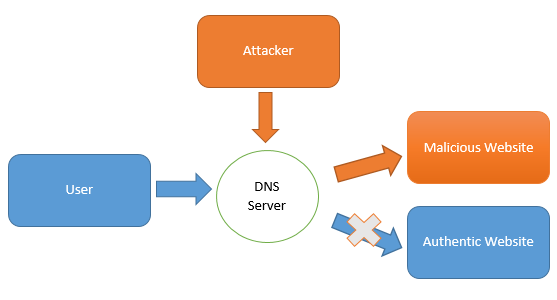
\includegraphics[width=0.8\linewidth]{images/dns.png}
  \caption{DNS attack}
  \label{img: dns}
\end{center}
\end{figure}
\subsubsection{BlackWallet.co}
On $13^{th}$ January of 2018, BlackWallet.co suffered from DNS Redirection attack. Adversaries redirected, the DNS entry of the BlackWallet.co domain, to a server they operated \cite{blackwallet_nodate}. As a result of that users were logging in malicious server, then attackers used that credentials to steal money from authentic wallet. Users lost around 6,70,000 Lumens which is one of the top ten cryptocurrency, contemporary worth of \$0.4 million. 
\subsubsection{Caution Against DNS Attack}
It is very difficult for normal user to interpret and confirm whether organization's DNS is hijacked or not, but as a active user, everyone can keep eyes on changes in website, application and unnecessary pop-up. Addition to that, organizations should post security related alert message on website to make users aware about potential threat to the system.
\subsection{DoS Attack}
In DoS (Denial of Service), adversary tries make network, framework or system unavailable for indefinitely with the intention of disruption in system \cite{chao-yang_dos_2011}. In most of the cases, this attack is done by doing excessive number of requests to the sytem, which can prevent query or request from authentic users \cite{dos_wireless_singh_denial_2017}. Well-known example of this attack is sending request to web server, which might result into the congestion in network and repudiation of request from some user. Such attack has a potential to damage blockchain framework also. For an example, a scenario in which nodes with malicious intention is part of network also. Now, malicious node can create unnecessary traffic in system. But it is very rare and difficult task in blockchain because of blockchain's dynamic topology\cite{zaghloul_beginners_2018}. In some cases, attackers use more than one node to send request in order do distributed attack, which is also known as DDoS \cite{saad_exploring_2019}. 
\subsubsection{Step Against DoS Attack}
Possibility of DoS can't be removed completely. However, there are some possible ways which can be used to curb DoS attack. Security of blockchain lies in the hashfunction with which blocks are related. One way to make blockchain secure is to reduce the size of block, but as size of block decreases number of transaction contained by single block also decreases. For security purpose, reducing the size of block is preferable. More number of block also increases transaction fees, that can be used to prevent DoS attack at some extent. Because while generating undesirable traffic on network, malicious nodes need to pay fees for each transaction. Size of block is parameters of the blockchain framework, by changing other parameters of the blockchain DoS attack can be controlled. Actually that method is trial and error method, researches are going on to find optimal result \cite{zaghloul_beginners_2018}. Ultimately, DoS attack is inevitable, but certainly ,by proper care chances of success can be reduced at large extent.       
\subsection{Sybil Attacks}
Sybil attack is kind of attack in which one person or entities tries to control whole network by pretending to many users at same time, this can be done by creating multiple account, nodes or computers \cite{zaghloul_beginners_2018}. In simple language, it can be compared to making multiple social media accounts. For the crytocurrency, relevant example for this attack is to make multiple nodes of blockchain network. In fact, large-scale sybil attacks, where attackers tries control most of the network is known as 51\% attack. 51\% is explained in section \ref{51attack}.
\subsection{Exchange Hack}
\cite{blockchainthreatreport}
\subsection{Orphaned blocks}
\cite{saad_exploring_2019}
\subsection{Eclipse Attack}
\cite{saad_exploring_2019}
\subsection{Consensus Delay}
\cite{saad_exploring_2019}
\subsection{Double-Spending}
\cite{saad_exploring_2019}
\subsection{Software Flaw}
%\section{Security Issues}
%Distribution of information and data among several computers residing at various locations removes %possibility of single node failure. In addition to that, use of ledger and hashing eliminates the issue of %hacking \cite{topfiveblockchainsecurityissues}. But, as mentioned below, Some issues are required to be taken %care, otherwise it might lead to repercussion.
%\subsection{Technical Limitations}
%Main idea of blockchain lies in storing redundant data at more one node. For the continuous updation is %mandatory, but for that complex network among participants.  
%\cite{fangfangdai}
%\subsection{Opensource BlockChain Platforms Attract Intensive Attacks}
%\cite{fangfangdai}
\subsection{Security Management of Self-organization and Anonymity}
\cite{fangfangdai}
\section{Security Risk}
Popularity and execution of any technology in industry relies on the effective risk management. Risk management becomes vital when Technology is core of the company. Blockchain is not an exception from them. Blockchain should be implemented correctly and effectively, so that it fulfills organization intention of data security, privacy, confidentiality and time efficient solutions.
\subsection{Standard Risks}
Organizations are vulnerable to the some standard risk even while using blockchain Technology. Such issues should be addressed for the efficient and successful use of blockchain \cite{securityrisk}. Below details about such typical risks are mentioned. 
\subsubsection{Planning Risk}
Resources, used for the implementation of blockchain, can be hindrance for the product and services being delivered from the platform of blockchain. In addition to that, organization should be careful while deciding which entities can participate in blockchain network. Because number of participation can create impact on the efficiency and security of blockchain.    
%\subsubsection{Business Continuity}	
\subsubsection{Reputational}
Most of the fintech applications of other technology are not the core of organization, whereas blockchain is heart for expansion and survival of institute. Failure of blockchain might leads to shut down of whole industry, and bad consumer experience.   
\subsubsection{Information Security Risk}
Firstly, as explained in \ref{typesofattacks}, blockchain is vulnerable to various cyberattacks such as 51\% attack, phishing, DNS hijacking, etc. 51\% attack is mostly dangerous for permissioned system. Secondly, user details such log in credentials, password is susceptible for attackers, who intent to take over user's account for malicious purpose. 	
\subsubsection{Technical Limitations}
Main idea of blockchain lies in storing redundant data at more one node. For the continuous updation is mandatory, but for that complex network among participants. It requires large scale network with huge computation power.  
\cite{fangfangdai}
\subsubsection{Regulatory}
In present, there is no regulatory compulsion for blockchain. But in the future, regulatory risk related is possible, such as whether to include international transaction or not, privacy and data protection concern for international transaction.    
\subsubsection{Operational and IT}
Current rule, regulations, procedure, law and policies needs to be changed to adapt new business methodology. In addition to that, there remains technological concern for catch up the demand of scalability and speed.   
%\subsubsection{Contractual}
%\subsubsection{Supplier}
\subsection{Value Transfer Risks}
Elimination of third party exposes communicating nodes to new risks, earlier these risks were controlled by trusted third party. In other word, there remains risk while transferring value from one node to another node. These value can be information, assets, and identity.
\subsubsection{Consensus Protocol}
The transfer of value between node occurs by agreement from other nodes which use consensus protocol, and
Proof-of-Stack and Proof-of-Work are consensus algorithms. Proof-of-Stack is consensus algorithm with the advantage of energy efficiency and security over Proof-of-Work \cite{saad_exploring_2019}. Deficient consensus protocol can lead to the fatal result. For an example, in the case of Proof-of-Stack, there is a chances of  problem called Nothing at Stack \cite{wiki:proofofwork}.  
\subsubsection{Data Confidentiality}
In distributed ledger technology, to fulfill the demand of system, data or information needs to be shared all over the network. Doing so result into the loss of confidentiality from basic requirements CIA (Confidentiality, Integrity and Availability). Monitory the metadata can revel a lot about the type of activity and volume associated with the activity of any public address.
\subsubsection{Key Management}
Though mechanism of blockchain makes it next to impossible to alter the block, chances of theft is private key is always there. Once private is exposed to the adversary, he/she can extract money using public key. So, when it comes blockchain's private key, precious and proper management of key becomes mandatory.
%\subsubsection{Assets}
%\cite{infinance}
%\subsection{Smart Contract Risks}
%\subsubsection{Business and Regulatory}
%\subsubsection{Legal Liability}
%\subsubsection{Enforcement of contract}
%\subsubsection{Information Security}
\chapter{Conclusion and Future Work}
\end{spacing}
\begin{appendices}
\end{appendices}

%----------------------------------------------------------------------------------------
%					Bibliography
%----------------------------------------------------------------------------------------
\bibliography{report}
\bibliographystyle{ieeetr}
\end{document}
